\documentclass{beamer}

\usepackage[brazil]{babel}
\usepackage[utf8]{inputenc}
\usepackage{graphicx}

\usetheme{Warsaw}
\usecolortheme{beetle}

\newcommand{\putat}[3]{\begin{picture}(0,0)(0,0)\put(#1,#2){#3}\end{picture}}

\begin{document}

	\title{Robô Explorador de Ambientes}
	\author{Luis Camargo \newline \  Marcelo Teider \newline \  Matheus Araujo}
	\institute{Universidade Tecnológica Federal do Paraná}

	\date{7 Dez 2011}

	\frame{\titlepage}

	\frame{
		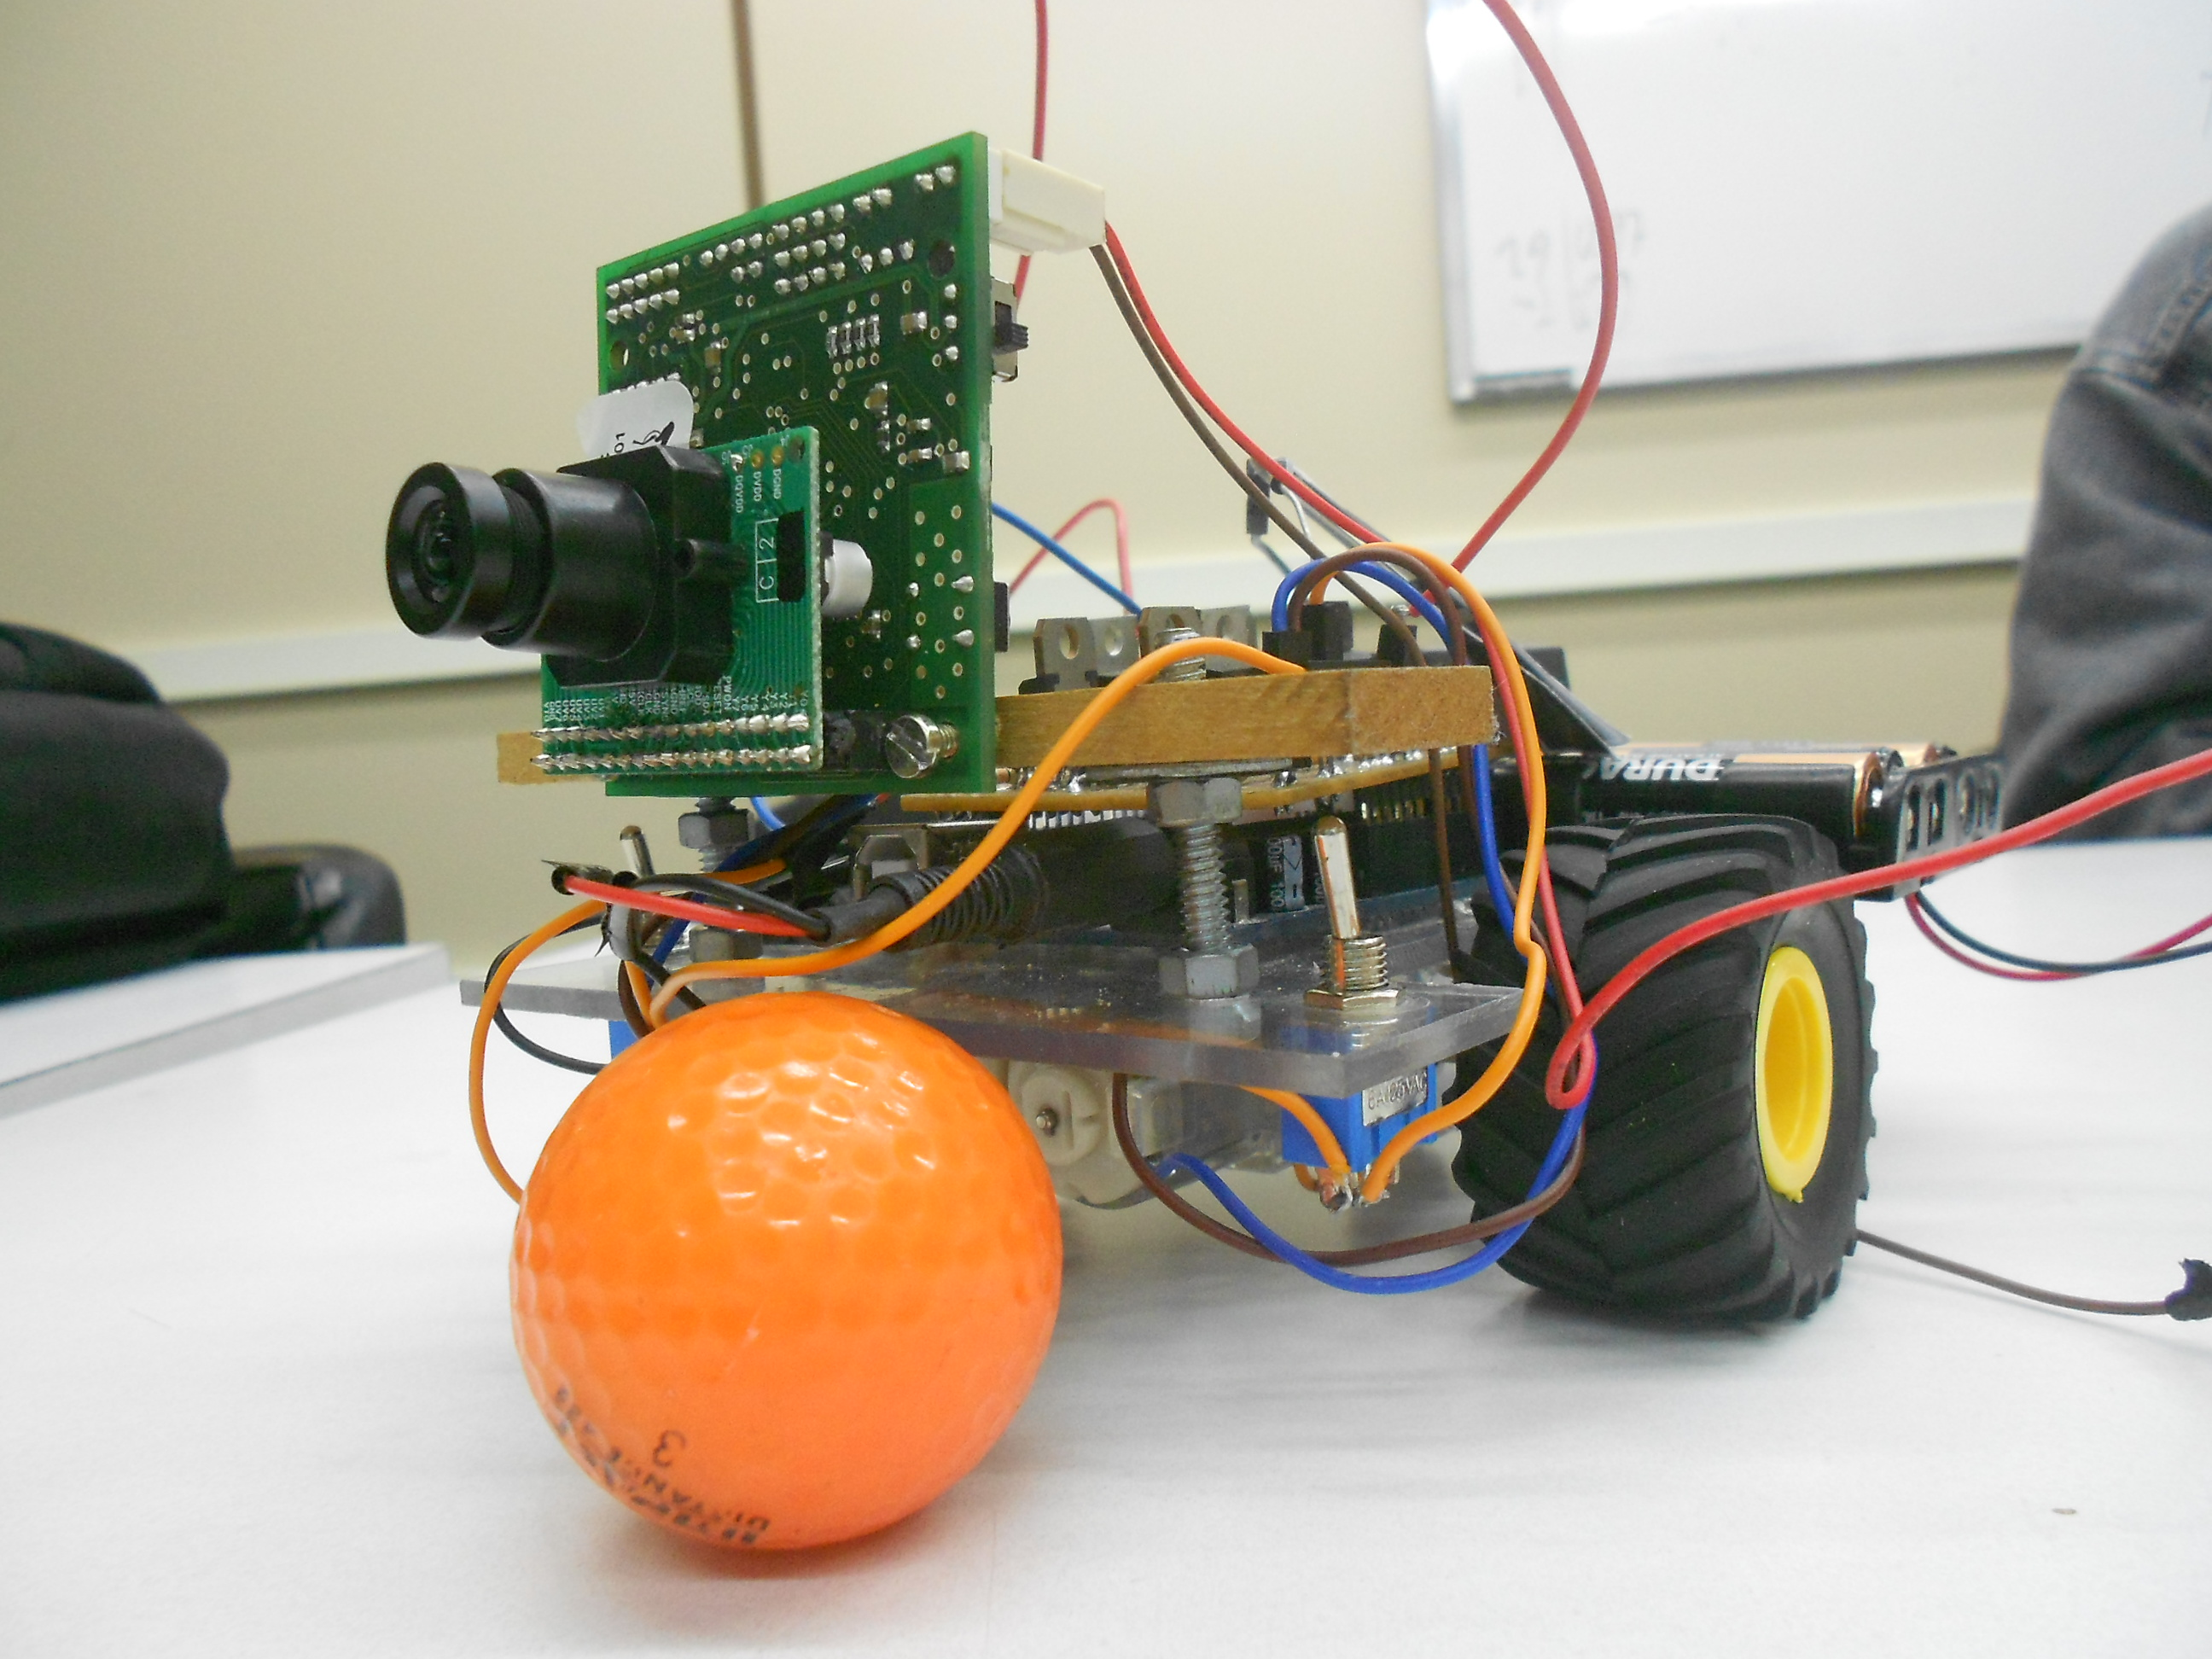
\includegraphics[width=11cm,height=7cm]{images/robo}
	}

	\section{Introdução}
	
	\frame{

		\frametitle{Introdução}
		
		\begin{itemize}
			
			\item \textbf{O que é?}

				\begin{itemize}

					\item Projeto de um robô que explora ambientes em busca de um objeto específico usando uma câmera como sensor.

				\end{itemize}

			\item \textbf{Por quê?}

				\begin{itemize}

					\item Porque é legal!

					\item Robôs exploradores têm diversas aplicações, desde atividades em hospitais a explorações espaciais.

				\end{itemize}
			
		\end{itemize}

	}

	\frame{

		\frametitle{Visão Geral}

		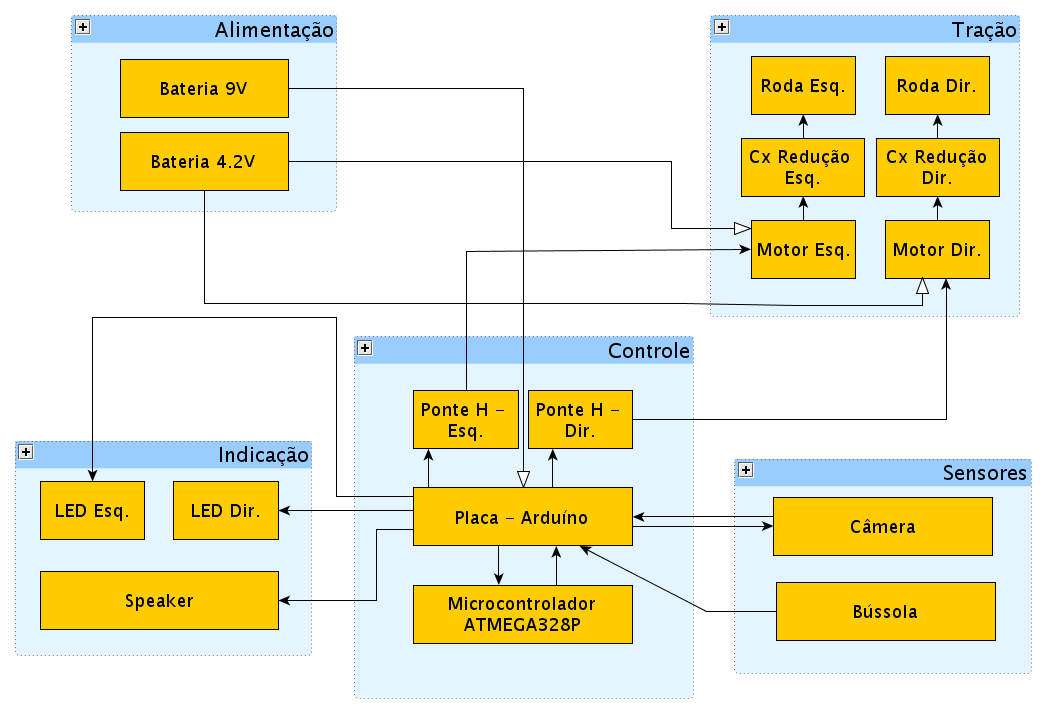
\includegraphics[width=11cm, height=7cm]{images/robo_geral}

	}	

	\section{Projeto Mecânico e Sensores}

		\frame{

			\frametitle{Projeto Mecânico}

			\begin{itemize}

				\item Robô construído no projeto \textbf{Robô Explorador de Labirintos 2D}, Bruno Meneguele, Fernando Padilha e Vinicius Arcanjo, apresentado a esta disciplina no primeiro semestre de 2011.

				\item Foram reutilizados: chassi, motor, caixa de redução, rodas, \textit{Arduíno}. 

				\item Os sensores de luz infravermelha foram substituídos pela câmera.

			\end{itemize}

		}


		\subsection{Robô}

			\frame{

				\frametitle{Robô}


				\begin{centering}

					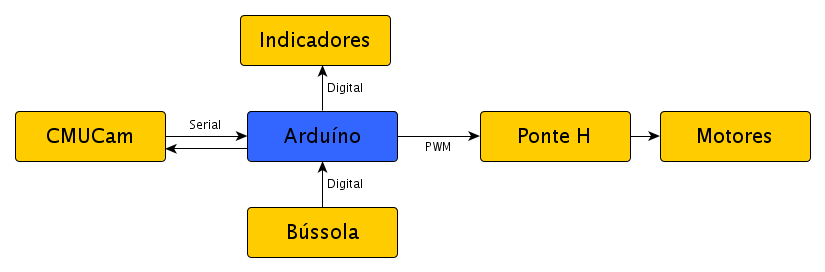
\includegraphics[width=7cm, height=3cm]{images/processo_arduino}

				\end{centering}


				\begin{itemize}


					\item O projeto do robô está centrado no \textit{Arduíno} - Ele é o responsável por receber as decisões tomadas pela câmera e atuar sobre os sistemas do robô.

					\item O acionamento dos motores é feito através da Ponte H, que por sua vez é ativada por PWM.

				\end{itemize}

			}
			
        \subsection{CMUCam}


			\frame{

				\frametitle{CMUCam}

				\putat{200}{-50}{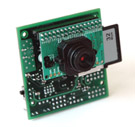
\includegraphics[width=3cm, height=3cm]{images/cmucam}}

				\begin{itemize}

					\item \textit{CMUCam3} - desenvolvida pela \\ \textit{Carmegie Mellon University}.

					\item \textit{Sensor inteligente.}

					\item Busca criar um sistema de visão simples que funcione em sistemas embarcados.

					\item Arquitetura baseada em \textit{ARM7TDMI}, Microprocessador \textit{Philips LPC2106}


				\end{itemize}

			}
                

		\subsection{Comunicação}

			\frame{

				\frametitle{Comunicação}

				\begin{itemize}


					\item Os algoritmos de visão e navegação são executados na \textit{CMUCam} e devem ser enviados para o \textit{Arduíno}.

					\item Foi utilizada comunicação serial assíncrona \textit{full-duplex} entre as duas plataformas.

					\item A \textit{CMUCam} envia um \textit{byte} contendo o movimento que deve ser executado pelo robô para o \textit{Arduíno} que o interpreta e executa.


				\end{itemize}

			}
			
		\subsection{Bússola}

		\frame{

			\frametitle{Bússola}

			\putat{210}{-20}{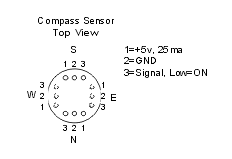
\includegraphics[width=2.75cm, height=2.5cm]{images/bussola1}}
			\putat{210}{-120}{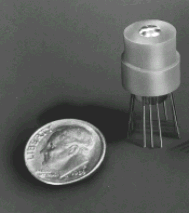
\includegraphics[width=2.75cm, height=2.5cm]{images/bussola2}}

			\begin{itemize}

				\item Apesar de não ter sido utilizada no \\ robô final, a equipe estudou e fez testes \\ com a bússola digital $Dinsmore \  \#1490$.

				\item Ela é capaz de fornecer a orientação \\ geográfica com 45 graus de precisão \\ através de quatro portas TTL.

			\end{itemize}

		}
		
    	\section{Exploração}

	
			\frame{

				\frametitle{Exploração}

				\begin{itemize}

					\item No início do projeto, foi proposto um algoritmo de navegação avançado que utilizaria uma percepção local do ambiente e então o exploraria.

					\item No entanto, devido a atrasos nas fases inicias do projeto, não foi possível implementá-lo a tempo desta apresentação.

					\item Foi implementado um algoritmo de navegação que encontra o objeto alvo, desde que ele esteja no campo de visão, e então move o robô até o mesmo.

				\end{itemize}
		
			}

		\subsection{Track-color}


		\frame{
			
			\frametitle{\textit{Track-color}}

			\begin{itemize}

				\item Programa presente na Biblioteca da \textit{CMUCam}.

				\item A função recebe uma faixa RGB definida e retorna as coordenadas de um retângulo com o centróide e a densidade de \textit{pixels} daquela cor presentes na imagem.

			\end{itemize}

		}

		\frame{

			\frametitle{\textit{Track-color}}

			\putat{10}{-20}{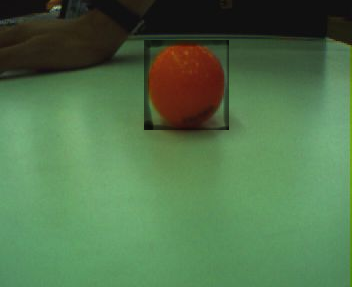
\includegraphics[width=5.5cm, height=3.5cm]{images/cam01.png}}

			\putat{150}{-90}{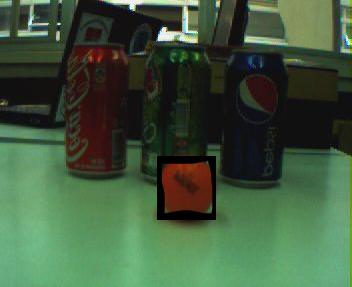
\includegraphics[width=5.5cm, height=3.5cm]{images/cam02.png}}

		}

		\subsection{Navegação}
	
		\frame{
		
			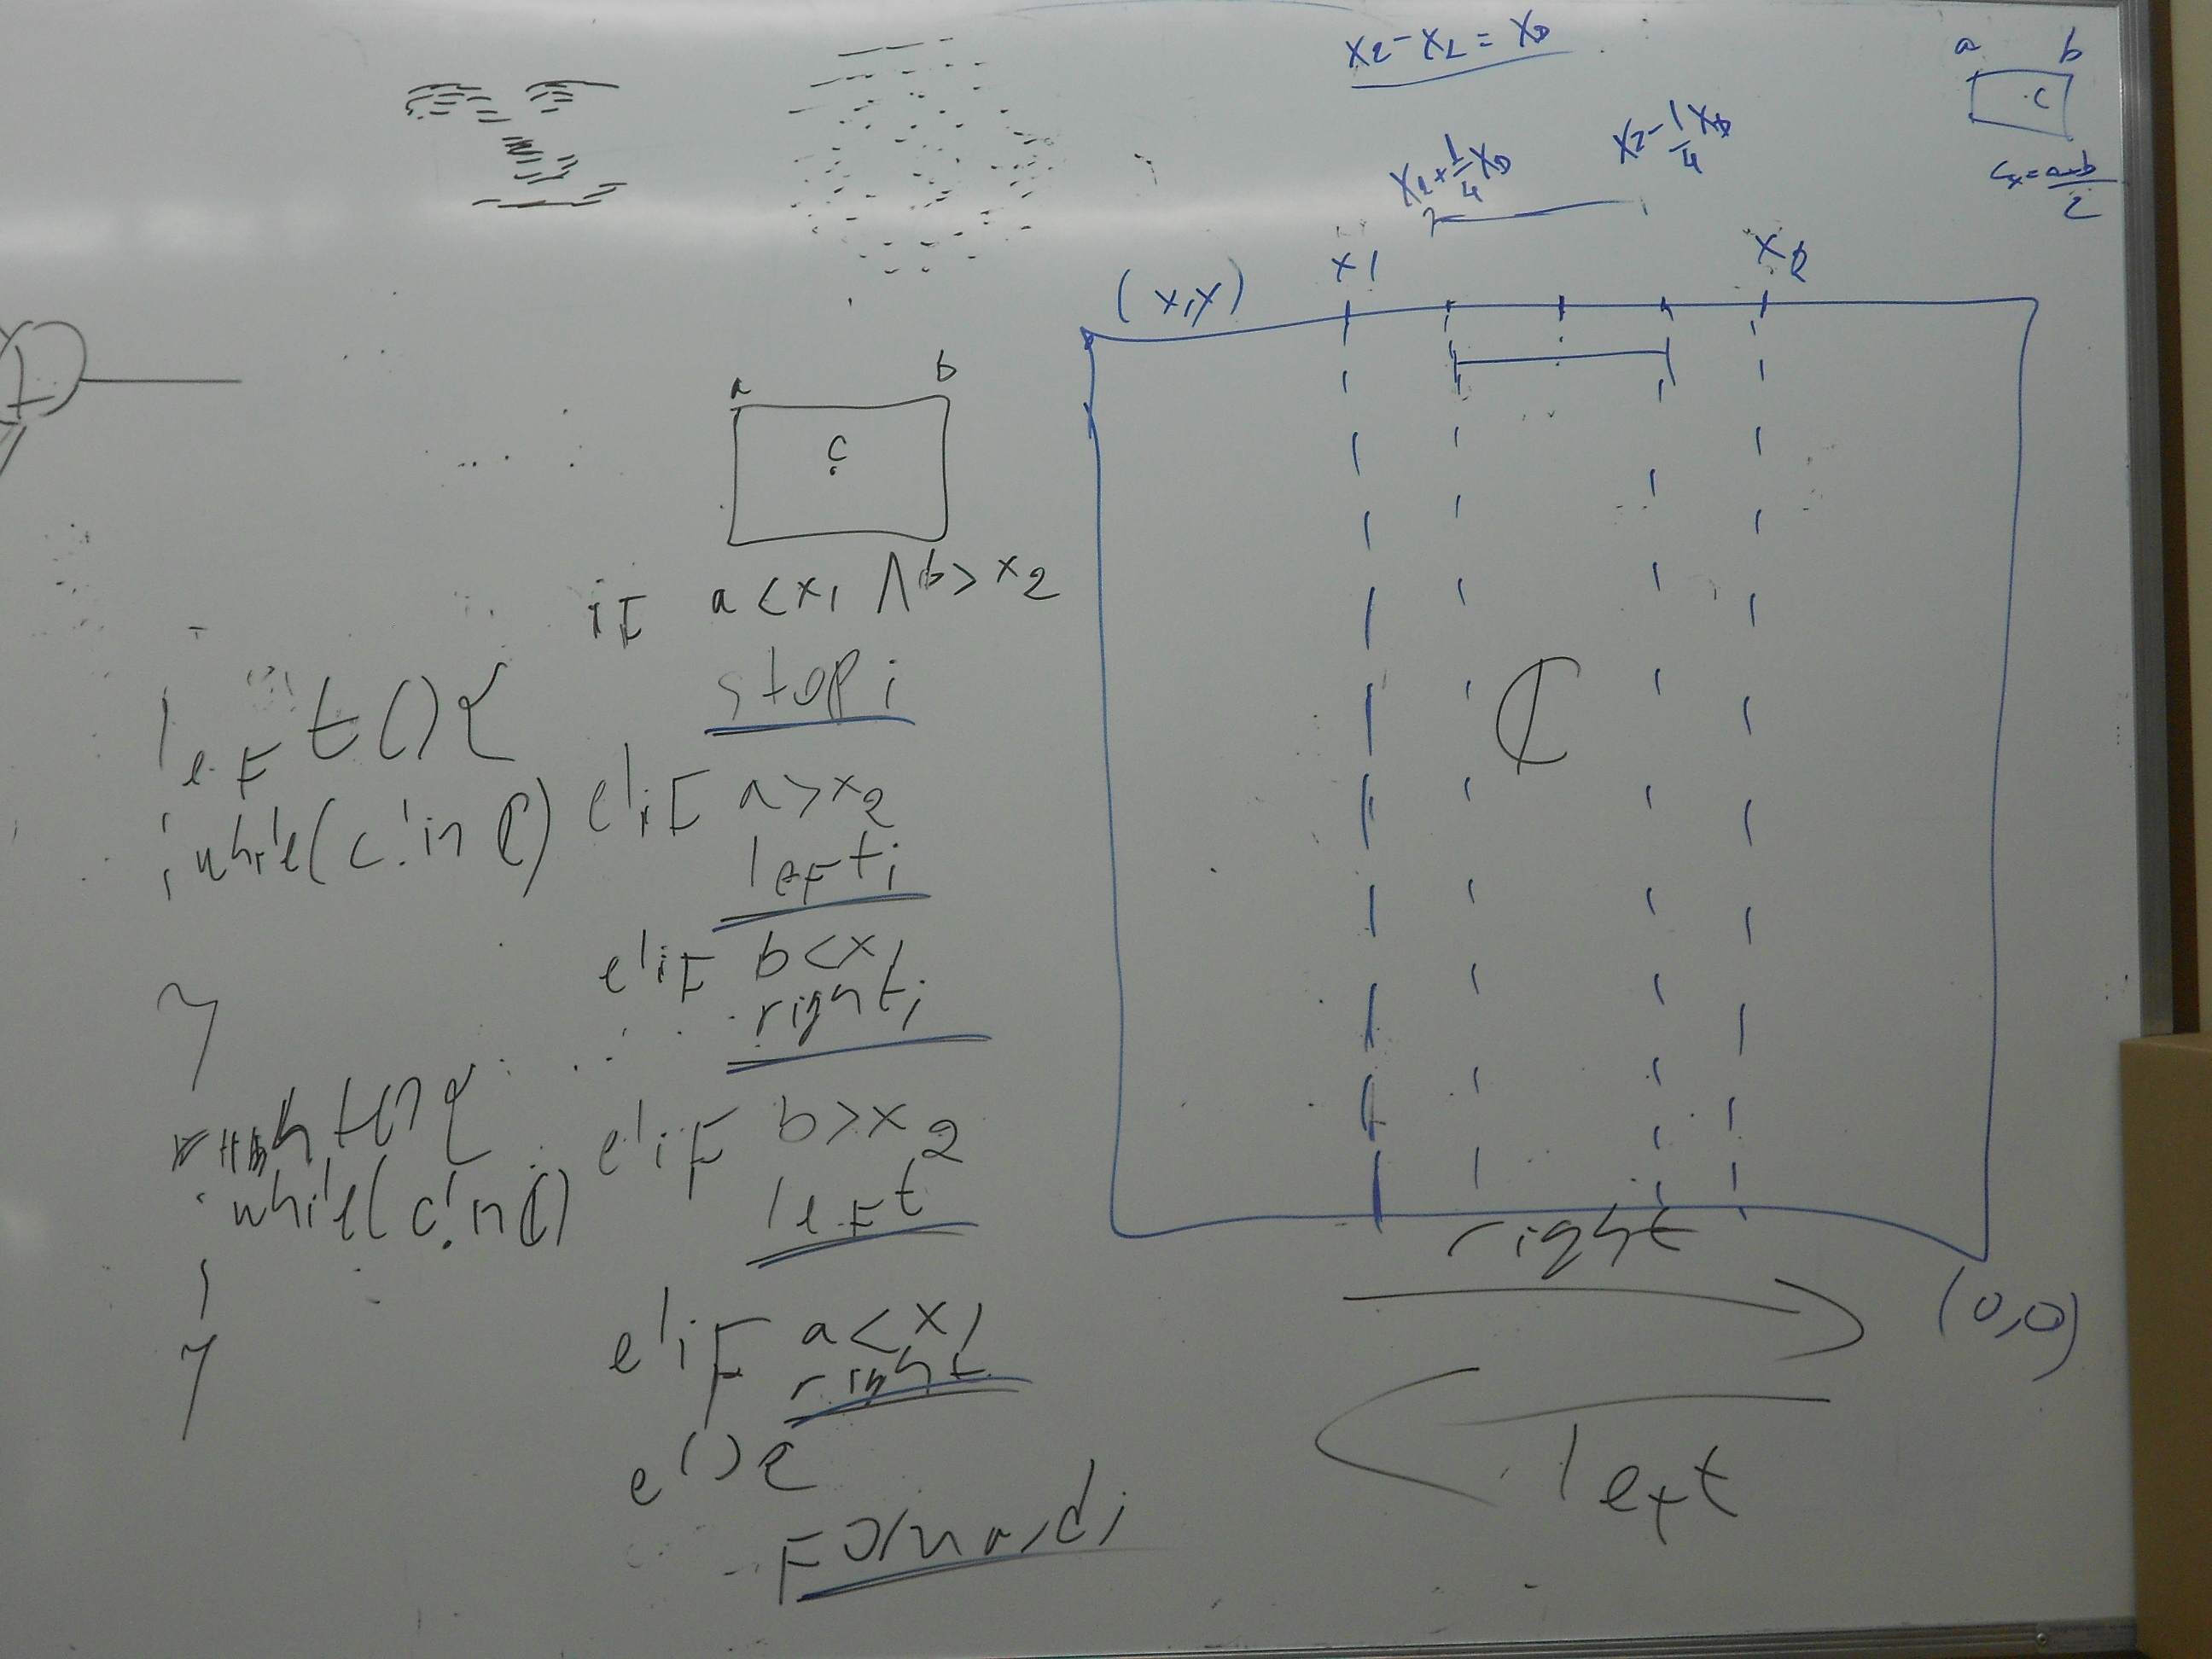
\includegraphics[width=11cm, height=7cm]{images/algoritmo_navegacao}
			
		}

		\frame{

			\frametitle{Exploração}

			\begin{itemize}

				\item O algoritmo de Exploração recebe as informações da função \textit{track-color} e toma a decisão de movimento do robô.

			\end{itemize}

		}

	\section{}

		\frame{
		
			\frametitle{Agradecimentos}

			\begin{itemize}

				\item Professores Myriam Delgado, Hugo Vieira, Mário Sérgio de Freitas, Cesar Tacla, João Fabro

				\item Colegas Bruno Meneguele, Fernando Padilha, Vinicius Arcanjo

				\item Colegas Claudio Akio, Kaya Sumire Abe, Lucas Paiva

				\item Marceneiros do Almoxarifado da UTFPR

			\end{itemize}
		
		}

		\frame{

			\begin{centering}

				Projeto disponível em:

				\vspace{1cm}

				\textit{http://github.com/matheusaraujo/oficina2-robocam}

				\vspace{1.5cm}

				\textbf{Boas Férias!}

			\end{centering}

		}



\end{document}
